%https://www.slideshare.net/maheshkha/cuda-tutorial (Memory space)
% https://www.slideshare.net/Hanibei/cuda-introduction - Kernel memory access
% https://www.microway.com/hpc-tech-tips/gpu-memory-types-performance-comparison/
%Husk at tjekke Shane Cook Hardware architecture afsnittet her.
%TODO Understanding NVIDIA GPGPU Hardware
%TODO Update to newest ( and consider all cahces)

As presented through the earlier sections, the GPU hardware architecture contains multiple types of memories \& caches.
As these individual types vary in size, speed, accessibility \& lifetime one must know their context and features.
This section provides a understanding of these different memory types, but as the other components within the architecture, these changes as well depending on the architecture version.
Therefore, the memory model presented in this section also is a conceptual model, with the focus of providing general understanding.
First the memory types are presented in \cref{sec-mem-types}, and hereafter the caches in \cref{sec-cac-types}.

\subsubsection{Memory types}
\label{sec-mem-types}
\textbf{Register File -} As presented in \cref{sec-hw-streaming-processors}, the Register Files are located in the SMs and used by SPs as registers.
Due to the SIMT execution model, a large number of threads are run on a SP at a given time.
This results in a high demand for a large volume of registers, which due to its large size is implemented by SRAMs \cite{Li2016}.
As described in \cref{sec-hw-warps-threads}, the Register File is shared between the different warps running on a SM.
To increase the allocation capabilities in this sharing, the registers within the Register File are not dedicated to specific cores, but instead potentially shareable by each thread.
On the execution of threads, the SM assigns registers to it, which are bound to the thread until its lifetime ends.
In this access binding, no other thread can access the register for read or write operations.
\\\\
\textbf{Local Memory -} The Local Memory it is actually a portion of the Global Memory.
It is therefore not as such a physical memory space but only a partition.
Differing from the Global Memory, its accessibility scope is per-thread just like the Register File.
It is generally used for \textit{register spilling}, meaning that if the amount of registers available in the Register File is insufficient for the amount of variables in the application, they are instead saved in the Local Memory.
Depending on the hardware architecture, the Local Memory is either cached by both the L1 and L2 Cache or only the L2 Cache.
The need of Local Memory due to register spilling reduces the performance greatly.
As illustrated on \cref{fig:hw-memory-schematic}, the Register File is the fastest memory accessible in the GPU. %Størrelses forhold fra hjemmeside.
Now, with register spilling, this speed is in best case reduced to the speed of the L1 and L2 Caches.
In the case of what is known as a cache miss, meaning that the data is unaccessible through the cache, the value must be fetched from the off-ch


As the Local Memory is located in the Global Memory, and thereby off-chip in regards to the SM,  
\\\\
\textbf{Shared Memory -} blabla
\\\\
\textbf{Global Memory -} blabla
\\\\
\textbf{Texture Memory -} blabla
\\\\
\textbf{Constant Memory -} blabla


\subsubsection{Cache types}
\label{sec-cac-types}
\textbf{L1 Cache -} blabla
\\\\
\textbf{L2 Cache -} blabla
\\\\
\textbf{Texture Cache -} blabla
\\\\
\textbf{Constant Cache -} blabla

\begin{table}[]
	\begin{tabular}{|l|c|c|c|c|c|}
		\hline
		\textbf{Memory}          & \textbf{On/Off Chip(SM)} & \textbf{Cached} & \textbf{Access} & \textbf{Scope} & \textbf{Lifetime} \\ \hline
		\textbf{Register File}  & On                   & N/A             & Read/Write      & Per-Thread     & Thread            \\ \hline
		\textbf{Local Memory}    & Off                  & L1/L2           & Read/Write      & Per-Thread     & Thread            \\ \hline
		\textbf{Shared Memory}   & On                   & N/A             & Read/Write      & Thread Block   & Thread Block      \\ \hline
		\textbf{Global Memory}   & Off                  & L1/L2           & Read/Write      & GPU+CPU        & Host Allocation   \\ \hline
		\textbf{Constant Memory} & Off                  & Constant Cache  & Read Only       & GPU+CPU        & Host Allocation   \\ \hline
		\textbf{Texture Memory}  & Off                  & Texture Cache   & Read Only       & GPU+CPU        & Host Allocation   \\ \hline
	\end{tabular}
	\centering
	\captionof{table}{GPU Memory Features \cite{Li2016}}
	\label{alg-gpu-mem}
\end{table}

\begin{figure}[H]
	\centering
	\fbox{
		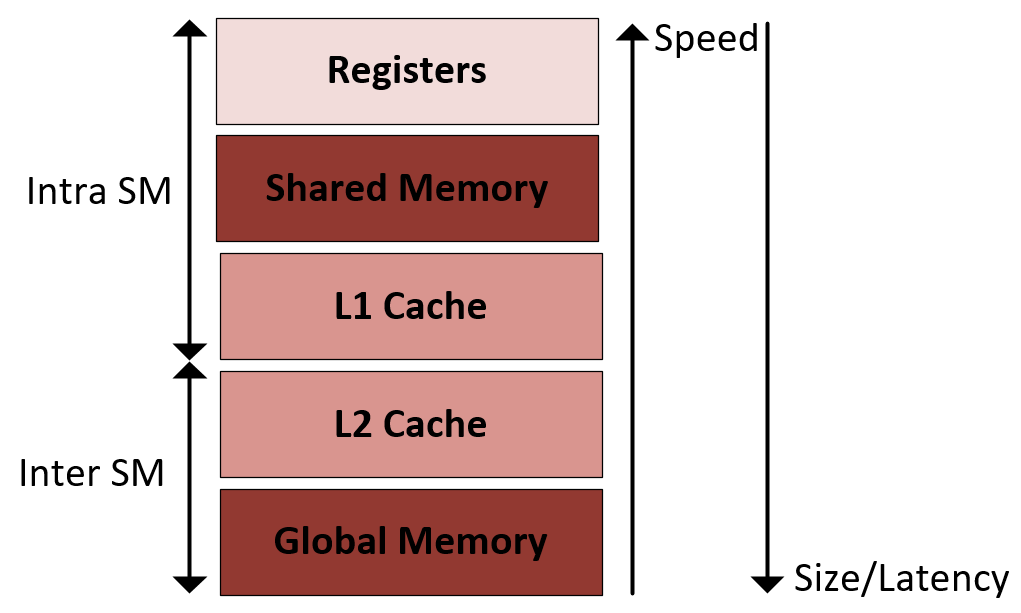
\includegraphics[width=0.6\textwidth]{figs/hw/hw-memory-schematic}}
	\caption{GPU memory schematic}
	\label{fig:hw-memory-schematic}
\end{figure}

\begin{figure}[H]
	\centering
	\fbox{
		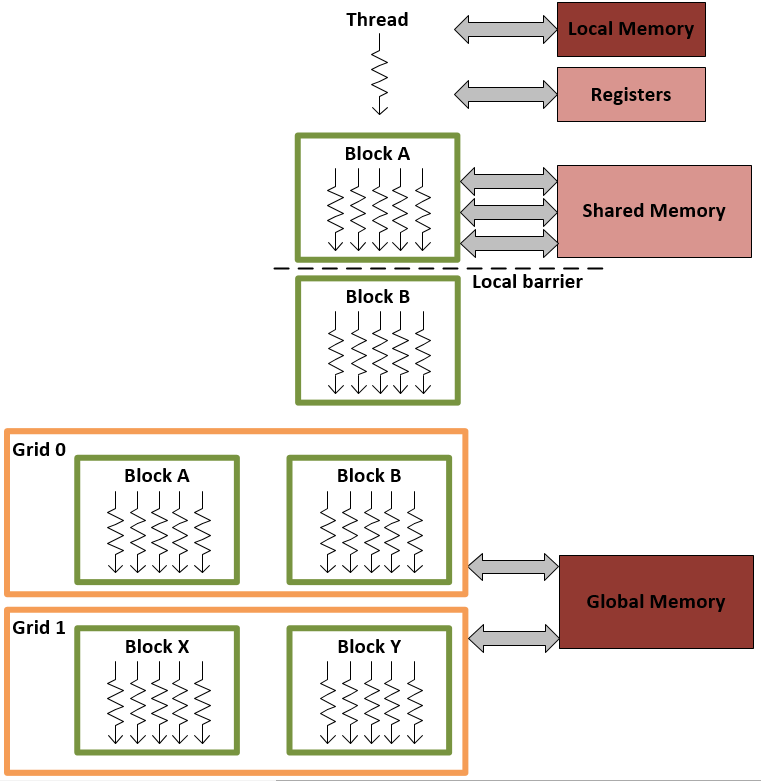
\includegraphics[width=1\textwidth]{figs/hw/hw-memory-model}}
	\caption{GPU memory access scopes}
	\label{fig:hw-memory-model}
\end{figure}

